\chapter{開発}	% TODO: 章題を記入.題は任意.
\thispagestyle{plain}   % chapterの直後に必ず指定

%TODO: 章の内容を記入.以下はサンプル.
本研究では,\ref{chap:minecraft}章で述べたMinecraftの特性に焦点を当て,Minecraftの中でLLMを搭載したBOTを作成し,そのBOTと人間が対話を行ったり,共同作業を行ったりすることで,人間とAIの協力・協調関係の検証を行う.

本章では作成したBOTについて解説する.
システムの全体像は図\ref{fig:system}のとおりである.
プレイヤーはBOTログイン用webアプリケーションを使用して,BOTをMinecraftのマルチサーバーに参加させることが可能である.
その後プレイヤーは,BOTが参加したマルチサーバーと同じサーバーにログインしMinecraftのチャットの機能(デフォルトでTキー)を用いてBOTと対話することができる.

マルチサーバーにログインしたBOTはプレイヤーからのチャットの情報をLLMに送り,LLMからの返答をもとにプレイヤーへ返答や行動を行うことが可能である.
詳細な機能については\ref{sec:webapp}節から\ref{sec:build_mode}節で解説する.

\begin{figure}[H]
    \centering
    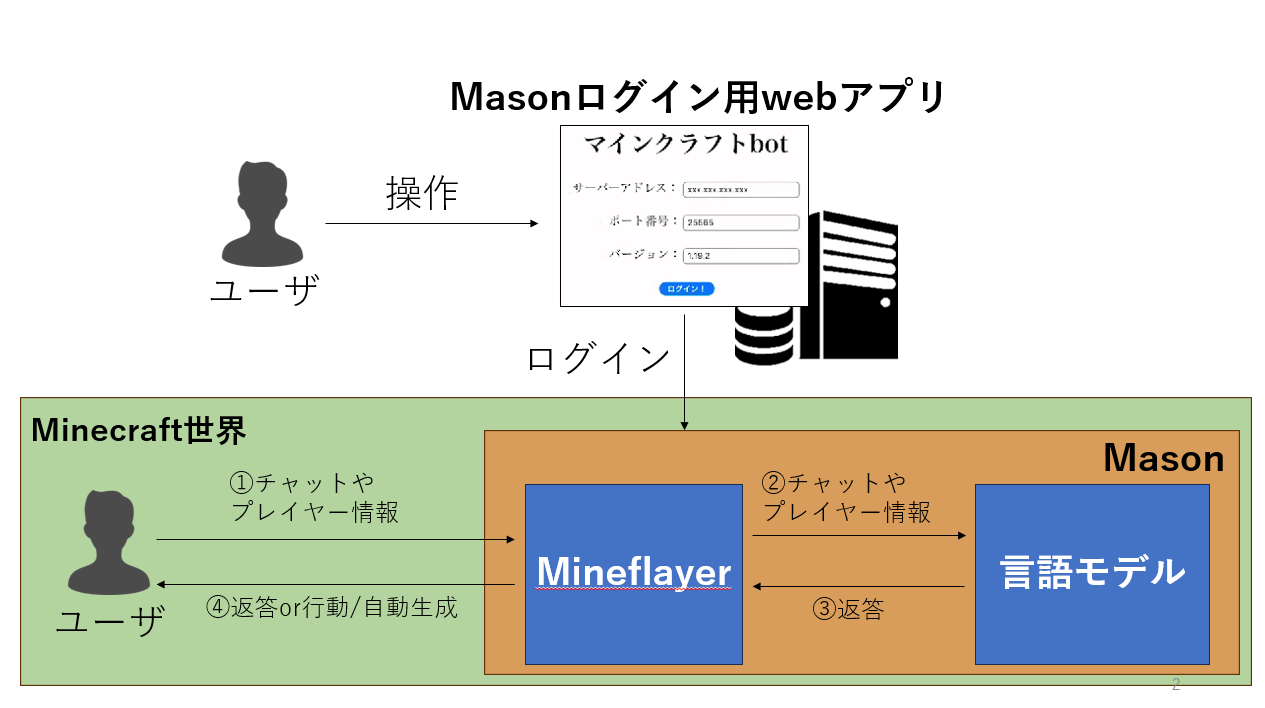
\includegraphics[width=0.8\textwidth]{fig/my_system.PNG}
    \caption{システムの全体像}
    \label{fig:system}
\end{figure}

\section{Webアプリケーション}\label{sec:webapp}
人間とAIの協力・協調を主目的とする以上,ユーザビリティについて追求する必要があると考えたため,BOTをログインさせるためのWebアプリケーションを作成した.
従来までの方法でBOTを動かすためには,プログラミング環境構築のスキルを必要とするが,このアプリケーションではマイクラのマルチにログインする時と同様の情報を入力することで,簡単にBOTをログインさせることが可能となった.

\begin{figure}[H]
    \centering
    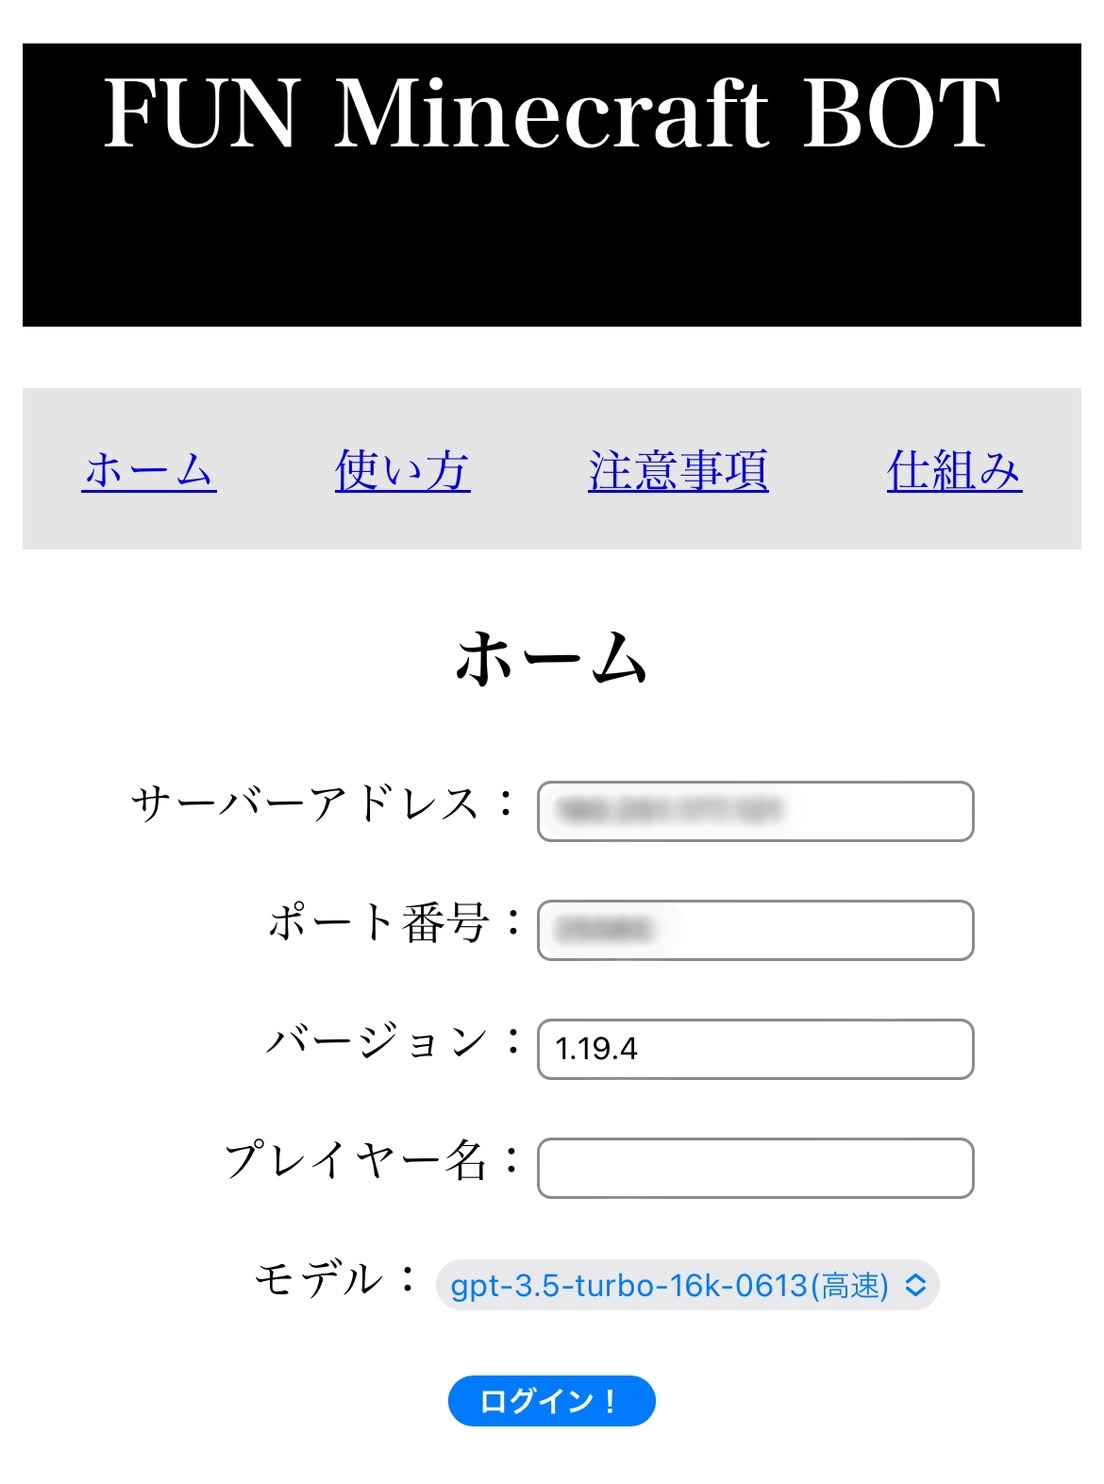
\includegraphics[width=0.5\textwidth]{fig/web_app.jpg}
    \caption{Webアプリケーションのホーム画像}
    \label{fig:web_app}
\end{figure}

\section{行動}\label{sec:act}
BOTは事前に登録されている行動を実行することが可能である.
BOTの各行動はMineflayer API\cite{bib:Mineflayer}を用いて実装した.
指定位置への移動,所持アイテムをチャット,アイテムの出し入れ,畑に種を植える,指定アイテムを収集する行動などを実行することができる.
また,\ref{sec:build_mode}節のビルドモードも行動として実行できる.

\section{ChatGPTによる応答}\label{sec:gpt_res}
BOTはLLMを搭載したことで自然な返答が可能となっている.
LLMはChatGPTやPaLM,ローカル環境で動作するDollyなどいくつかのモデルを検討し,実行速度,会話の自然さや機能面の観点から自己検証を行ったところChatGPTが良かったことから,ChatGPT(gpt-3.5-turbo-0613)を用いた.

初期プロンプトはVoyager\cite{bib:Voyager}のものを一部参考し,内容としてはChatGPTの役割,各会話のラウンドで与える情報,回答の際に守るべきルールを記載した.
また,ChatGPT APIのFunction Calling機能を用いているので,\ref{sec:act}節の行動を,必要に応じて実行することが可能である.

\section{ビルドモード}\label{sec:build_mode}
BOTは``建築したい''などのチャットを受け取るとビルドモードに移行し,Minecraftの/fillコマンドを用いてChatGPTがプロンプトに沿った構造物を生成することが可能である.

初期プロンプトには,/fillコマンドで構造物を生成すること,/fillコマンドの説明,3次元座標の概念の説明,よく建築で使うブロックの種類,/fillコマンドの使用例を記述した.
